\chapter{Zukünftige Entwicklungsmöglichkeiten}
Obwohl das Praktikum erfolgreich verlief, werden in diesem Kapitel noch Verbesserungsvorschläge und Ausbaumöglichkeiten beleuchtet. 

\section{Regler}
Die Messwerte des Gyroskops können für einen Regelkreis (Abb.~\ref{bild:regler}) benutzt werden. 

\begin{figure}[!ht]
	\centering
	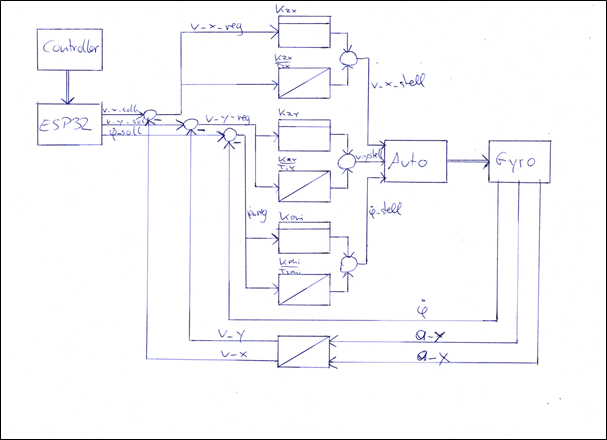
\includegraphics[width=\textwidth]{bilder/regler.png}
	\caption{Blockschaltbild Regler}
	\label{bild:regler}
\end{figure}

Durch die Eingaben des Spiele-Controllers und deren Interpretation durch das ESP-32 werden Sollwerte für Geschwindigkeiten in allen Achsen vorgegeben. 
Das Gyroskop misst Beschleunigung in X- und Y-Richtung und die Winkelgeschwindigkeit der Rotation. 

Deswegen müssen die Beschleunigungswerte einmal integriert werden, um auf die momentane Ist-Geschwindigkeit in beiden Richtungen zu kommen. 
Das übernimmt der Integrator ganz unten. 

Anschließend wird von den Soll- und Ist-Werten die Differenz gebildet. 
Über diese Regelungsdifferenz wird jeweils durch einen PI-Regler (Proportional und Integrationsglied) mit empirisch bestimmten Faktoren die Stellgröße ermittelt. 
Das Integrationsglied der PI-Regler ist dabei wichtig für die stationäre Genauigkeit. 

Die Stellgrößen werden nach Umrechnung an die Motoren weitergeleitet, was wiederum zu veränderten Messgrößen am Gyroskop führt. 
Damit ist der Kreis geschlossen. 


\section{Verbesserungen}
Stillstand bedeutet Rückschritt. Daher werden bei zukünftigen TEGGLA Versionen sowohl Hardware als auch Software Komponenten angepasst, um jedes Fahrzeug besser als dessen Vorgänger zu machen.

\subsection{Hardware}
Für das omnidirektionale Fahren mit den Mecanum Rädern sind Stepper-Motoren besser geeignet als die aktuell verwendeten DC-Motoren, da diese eine vorgegebene Drehzahl besser halten können. Daher werden zukünftige TEGGLAs mit vier Stepper-Motoren ausgestattet sein.\\

Eine weitere hardwarenahe Verbesserung ist die Neugestaltung des Hauptschalter am Rahmen des Fahrzeugs. Dieser ist aktuell so konstruiert, dass der Hauptschalter bei einer Kollision des Fahrzeugs mit Objekten unbeabsichtigt betätigt werden kann. Daher wird in der nächsten Version des TEGGLA der Hauptschalter nach innen zeigen, um vor Kollisionen und unerwünschten Auslösen geschützt zu sein.\\

Die Verbesserung des Planetengetriebes ist zwar ein zeitaufwändiges Vorhaben, jedoch würde sich das ebenfalls positiv auf die Übersetzungsrate und somit auf das Fahren auswirken. Durch das Anpassen von Stellgrößen im CAD Modell und durch einige Druckversuche kann immer weniger Spiel im Getriebe erreicht werden. Eine Alternative wäre die Verwendung eines besseren, genaueren 3D-Druckers, da beim 3D-Druck eines Planetengetriebes bereits sehr geringe Druckungenauigkeiten problematisch sind.\\

Die vorerst letzten hardwarenahen Verbesserungsmöglichkeiten beziehen sich auf den Ladestecker und die Rollen der Mecanum Räder. Der aktuell verwendete Ladestecker (XT60) ist für ein häufiges Aufladen des Fahrzeugs nicht gut geeignet, da sich das Kabel schwer ein- und ausstecken lässt.\\

Die Rollen der Mecanum Räder sollen bei zukünftigen Versionen des TEGGLA mehr Grip haben, was eventuell durch die Verwendung eines anderen Filaments erreicht werden kann.\\


\subsection{Software}

Die Weboberfläche für die Kommunikation und Steuerung des TEGGLA soll fortlaufend erweitert und verbessert werden. 
Beispielsweise kann durch das Integrieren der Beschleunigung, welche vom Gyroscope gemessen werden, zusätzlich auch noch die aktuelle Geschwindigkeit des TEGGLA angezeigt werden.\\

Eine weitere softwarenahe Verbesserung des TEGGLA wäre das Beheben von Verbindungsproblemen. 
Bei dem Testen des fertigen Fahrzeugs kam es teilweise zu Verbindungsabbrüchen zum WLAN des TEGGLA. 
Dadurch konnte das Fahrzeug natürlich nicht mehr gesteuert werden und zusätzlich wurde der letzte erhaltenen Befehl dauerhaft ausgeführt. 

Dieses Verbindungsproblem kann durch zwei Schritte verbessert werden: Vorerst sollte der Code so angepasst werden, dass bei einem Verbindungsabbruch kein Befehl mehr ausgeführt wird und der TEGGLA somit keine unkontrollierten Bewegungen durchführt. 
Anschließend können automatische Reconnects implementiert werden, welche bei einem Verbindungsabbruch in kleinen Zeitabständen versuchen, die Verbindung automatisch wiederherzustellen. 
Dadurch kann die Zeit ohne Verbindung mit dem TEGGLA minimiert werden.
